\chapter{Background \label{sec:background}}

\noindent
This chapter collates the necessary background information for the project, including the fundamentals of passive radar, the use of illuminators of opportunity, range doppler mapping, radio hardware, digital signal processing, IoT architecture, and networking with embedded hardware.


\section{Passive Radar Fundamentals}
The key and unique feature of passive radar is its utilisation of existing illuminators of opportunity, such as television or radio broadcasts, to detect and track objects. The technology has been around since the early 20th century, with modern interest accelerated due to the use of passive radar systems on UHF TV signals and VHF FM radio tranmission systems in the 1980's \cite{FundamentalsPassiveRadar}. Equivalent terms used to describe passive radar include passive coherent location (PCL), and passive covert radar (PCR), parasitic radar, piggyback radar. Specifically, \textit{bistatic} radar refers to the distributed design of the transmitter and receiver, as opposed to classic \textit{monostatic} radar. As reflectd by Figure \ref{fig: topology} below, the turning parabolic of monostatic radar is able to receive both range and bearing of the signal echo, whereas passive bistatic radar measures time delay of the echos from the target, allowing doppler shift from the relative speed of the target to be measured.

\begin{figure}[htbp]
    \centering
    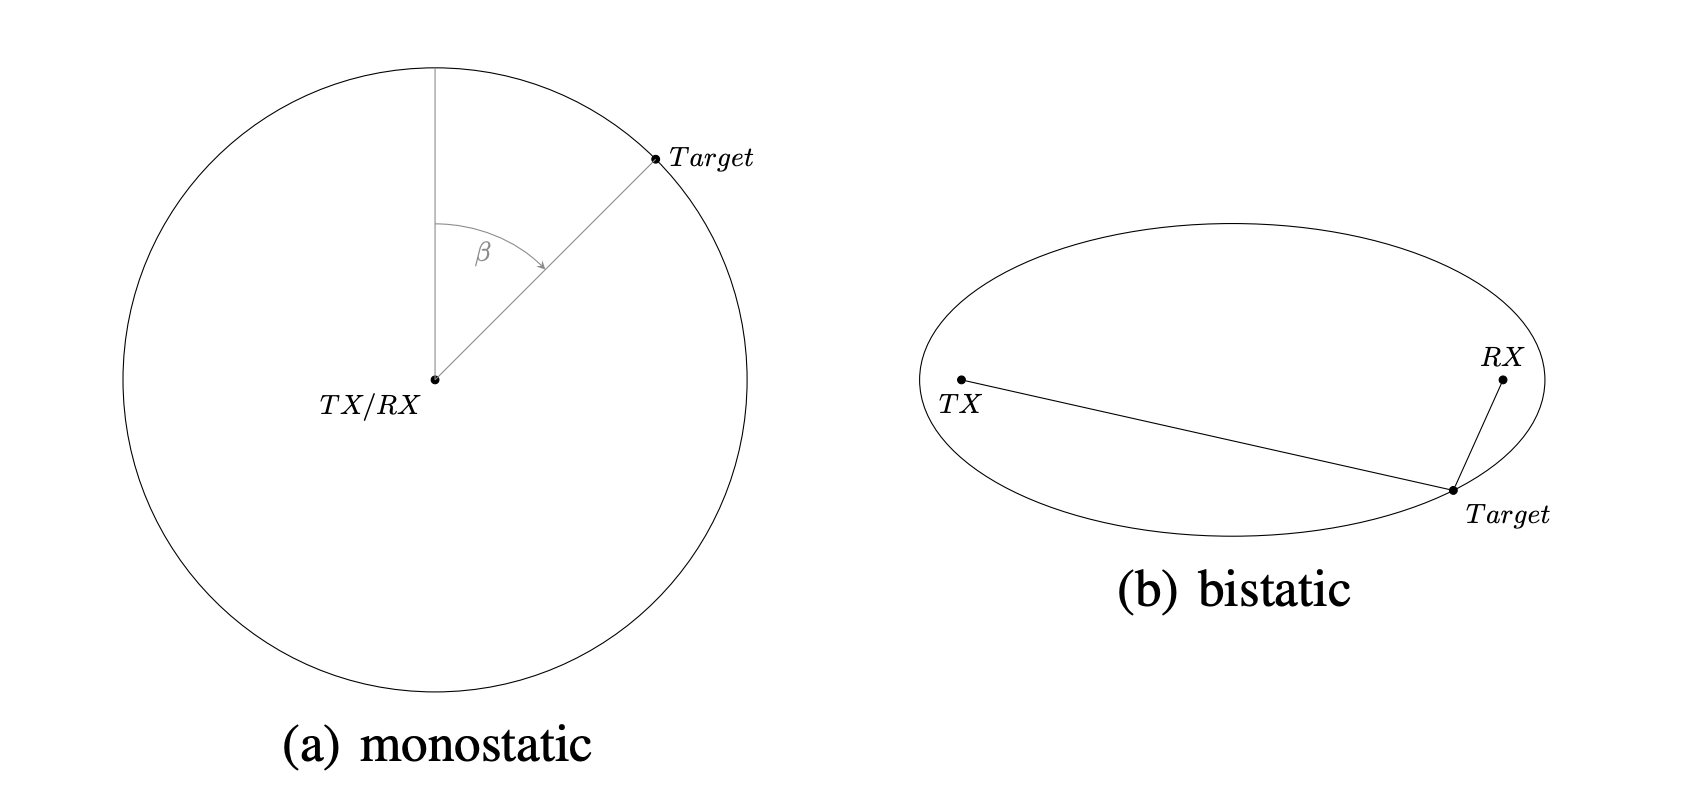
\includegraphics[width=0.8\textwidth]{monoBi.jpg}
    \caption{Monostatic (a) and bistatic (b) radar topologies \cite{IOTpassiveRadar}}
    \label{fig: topology}
\end{figure}

\par 
\vspace{0.5cm} 
\noindent The geometry of passive bistatic radar can be further explored and equations can be mapped accordingly, with the distance between the transmitter and receiver \textit{R} being determined by known quantities such as the baseline as reflected below in Figure \ref{fig:geometry}.


\par \vspace{0.5cm} 
\noindent The bistatic range \( R_R \) is given by:
\begin{equation}
R_R = \frac{(R_T + R_R)^2 - L^2}{2(R_T + R_R + L \sin \theta_R)}
\end{equation}

\noindent The Doppler shift \( f_D \) is given by the rate of change of the bistatic range sum:
\begin{equation}
f_D = \frac{1}{\lambda} \frac{d}{dt}(R_T + R_R) \xrightarrow{} f_D = \frac{2v}{\lambda} \cos \delta \cos(\frac{\beta}{2})
\end{equation}
In the case of this project, both the TX (illuminator of opportunity) and the RX (embedded passive detection system) will be static, and the target will be moving, simplifying the mathematical calculations as much as possible, resulting in the cos version of equation 2 above. 

\par
The Doppler shift will be used to determine the speed of the target as well as its relative directional motion, and the range will be used to determine the distance of the target from the receiver. Another important feature of bistatic passive radar systems is its performance which can be equated through the bistatic radar equation, which is equivalently derived as the monostatic radar equation \cite{FundamentalsPassiveRadar}. 
\vspace{0.5cm} 
\begin{equation}
    \frac{P_r}{P_n} = \frac{P_t G_t}{4\pi R_T^2} \cdot \sigma_B \cdot \frac{1}{4\pi R_R^2} \cdot \frac{G_r \lambda^2}{4\pi} \cdot \frac{1}{k T_0 B F}
\end{equation}
Where:
\begin{multicols}{2}
    \begin{itemize}
    \item \( P_r \) is the received target echo power.
    \item \( P_n \) is the receiver noise power.
    \item \( P_t \) is the transmit power.
    \item \( G_t \) is the transmit antenna gain.
    \item \( R_T \) is the transmitter-to-target range.
    \item \( \sigma_B \) is the target bistatic radar cross section.
    \item \( R_R \) is the target-to-receiver range.
    \item \( G_r \) is the receive antenna gain.
    \item \( \lambda \) is the signal wavelength.
    \item \( k \) is Boltzmann’s constant (\( 1.38 \times 10^{-23} \) JK\(^{-1}\)).
    \item \( T_0 \) is the noise reference temperature.
    \item \( B \) is the receiver effective bandwidth.
    \item \( F \) is the receiver effective noise figure.
    \end{itemize}
\end{multicols}

\begin{figure}[htbp]
    \centering
    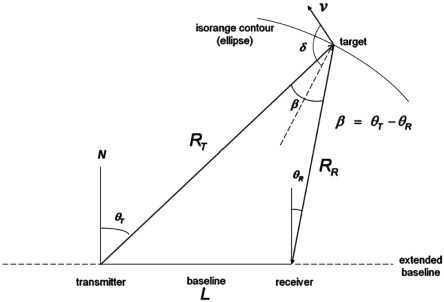
\includegraphics[width=0.8\textwidth]{geomPR.jpg}
    \caption{Bistatic radar geometry \cite{FundamentalsPassiveRadar}}
    \label{fig:geometry}
\end{figure}

\par \vspace{0.5cm}
\noindent The denominator of the bistatic radar equation includes the term \( \frac{1}{R_T^2 R_R^2} \).This term implies that with omnidirectional antenna patterns, the contours of constant signal-to-noise ratio (SNR) are described by the equation \( R_T R_R = \text{constant} \), which represents Ovals of Cassini. These ovals represent the locations in a given PBR co-ordinate sytem where the distances from the target to the transmitter and receiver remain the same. In the case of directional antennas, these contours are altered. Moreover, the signal-to-noise ratio is minimized when the target is equidistant from the transmitter and receiver (\( R_T = R_R \)), and maximized when the target is closer to either the transmitter or receiver \cite{FundamentalsPassiveRadar}.

\par \vspace{0.5cm} 
\todo[inline]{NEED TO MENTION / RESEARCH THE EFFECT OF NOISE AND DECIBELS EXPECTED HERE.}

% -------------------------------------------------
\section{Illuminators of Opportunity} %add label
\label{sec:illuminators}

The illuminator of opportunity is the signal that is used to illuminate the target, and is the primary source of the signal that is received by the passive radar system. The illuminator of opportunity can be any signal that is transmitted through the air, such as television radio or even satellite broadcasts, and can be tailored to the specific requirements of the passive radar system. Firstly it is necessary to comprehend the relevant radio frequency spectrum, followed by relevant metrics for passive radar, along with the advantages of digital signals.
\subsection{Radar and the Radio Frequency Spectrum}
% Image and description of the radio frequency spectrum
All wireless digital and analog signals are transmitted via a carrier frequency occupying some portion of the radio frequency spectrum. Each country regulates the use of the radio frequency spectrum, and the Australian Communications and Media Authority (ACMA) is responsible for regulating the radio frequency spectrum in Australia. The radio frequency spectrum is divided into bands, each with a specific range of frequencies, and each band is allocated for a specific use, such as television, radio, or emergency communcations. The spectrum allocation chart for Australia is shown in Figure \ref{fig:radioSpectrum} below. In general, radar systems are capable of operating across the entire radio frequency spectrum, with the specific frequency band chosen depending on the application and the desired range and resolution of the radar system. For example, Lockheed Martin have products suited to Low Band (VHF / UHF - 30-2Ghz) which is effective for long range detection, the midband (S/C - 2-8GHZ) and the high band which is not optimal for range but resolution \cite{LockheedRadar}. The below chart shows the Australian HF to UHF, with red reflecting potential illuminator signals.

\begin{figure}[htbp]
    \centering
    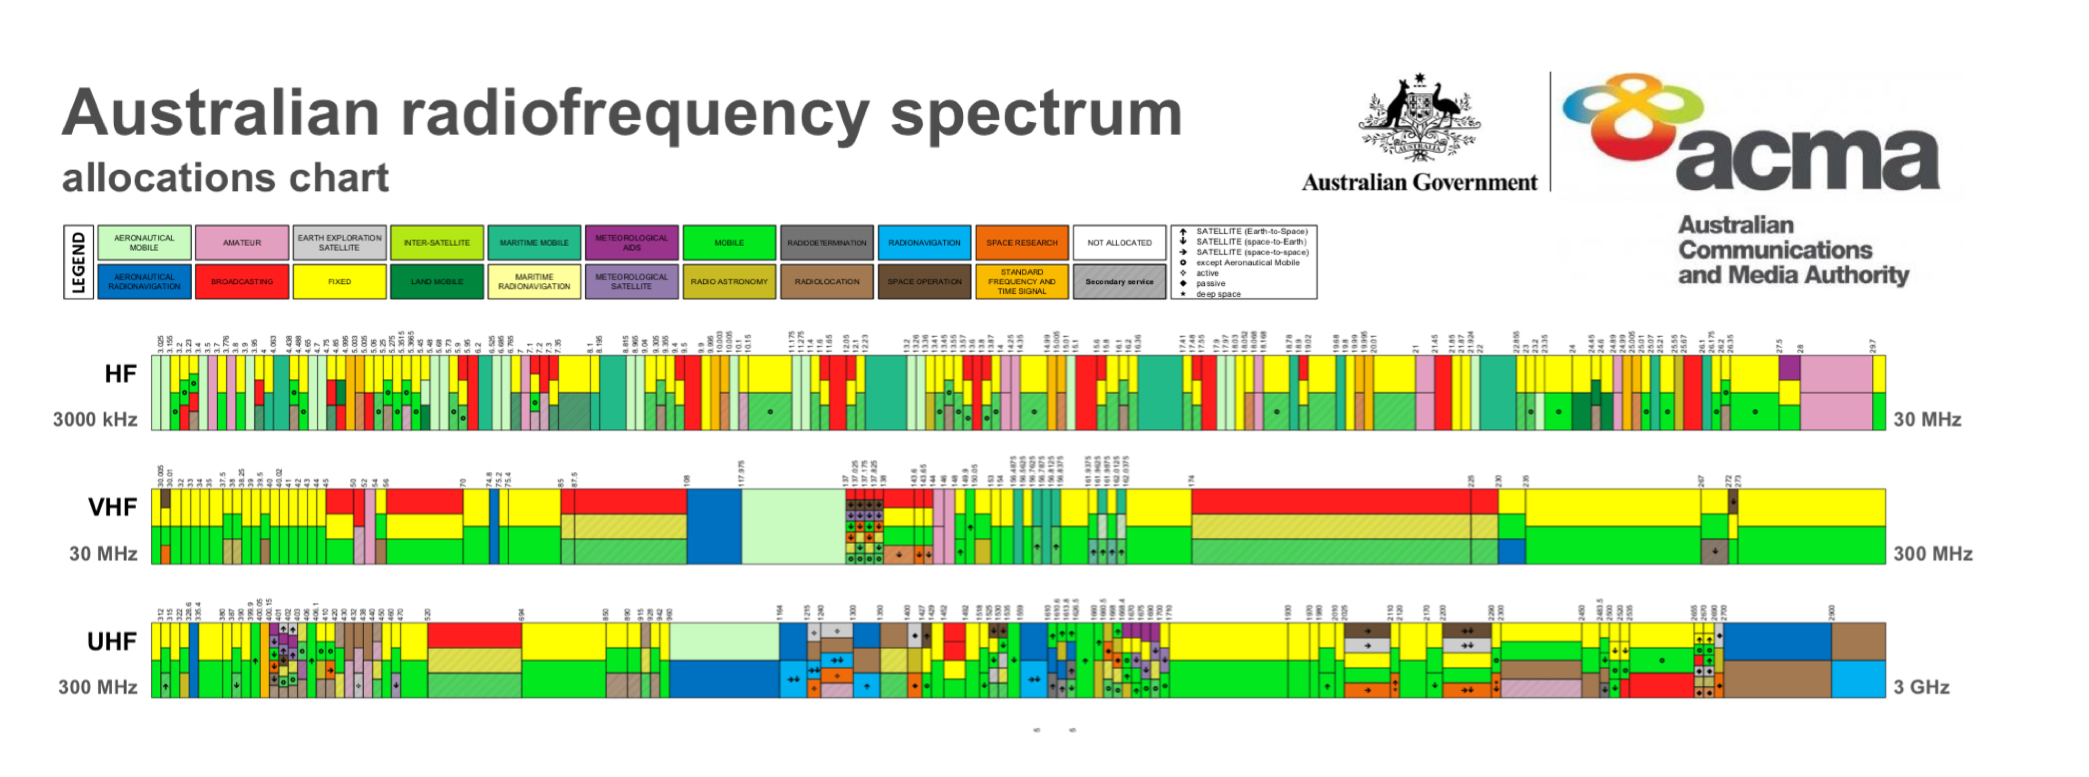
\includegraphics[width=0.95\textwidth]{ACMAspectrum.png}
    \caption{Australian radio frequency spectrum allocation HF to UHF \cite{SpectrumImage}}
    \label{fig:radioSpectrum}
\end{figure}

In the context of passive radar, the above three bands are relevant, firstly, due to the sheer volume of broadcast signals across the HF and VHF, representing a continuous source of illumination. Moreover, most of these signals have relatively high transmit power (with transmitters geolocated to facilitate maximum coverage for a given area), enabling clear reflections from targets \cite{DTSO2009}.

\subsection{Key Parameters for Illuminators of Opportunity}
Griffiths and Baker outline the three key paramaters when selecting an illuminator \cite{INTRO2017}:
\begin{enumerate}[label=\arabic*.]
    \item The \textbf{Power Density} at the target: It refers to the strength of the signal (in Watts per square meter) that reaches the target area from the illuminator. Higher power density can improve detection performance due to a stronger return signal.
    \item The \textbf{Nature of the Waveform}: This includes the waveform's properties, such as bandwidth and modulation, which can affect the radar's resolution and ability to distinguish between targets and clutter. The nature of the waveform can also be impacted by the program contents of the illuminator signal, for example, the waveform of FM broadcasts is noticeable different if the broadcast is music or speech.
    \item The \textbf{Coverage}: The spatial area over which the illuminator's signal is spread. Adequate coverage is essential to ensure the target is within the illuminator's effective range. As mentioned above, public broadcast signals are often optimized for a given locality.
\end{enumerate}

\subsection{Utility of Digital Illuminators}
In general, digital signals are favourable for passive radar due to their large bandwidth, constant envelope and relatively large and stable transmit power. Relevant Australian terrestrial analog signals for use in passive bistatic radar include Amplitude Modulation (AM) radio, Frequency Modulation (FM). Conversely, relevant Australian digital signals include Digital Audio Broadcasting (DAB) and Digital Video Broadcasting (DVB) \cite{DABfeatures}. With DVB-T being similar to DAB with a higher bandwidth and power, potentially resulting in more signal processing steps can be required as shown by Yin et. al \cite{DVBnoise}. The images below show the ambiguity functions of two equivalent frequency band signals, DRM (low frequency digital radio broadcast) and AM radio. The DRM signal has a much wider bandwidth, and a more constant envelope, which is advantageous for passive radar systems.

\begin{figure}[htbp]
    \centering
    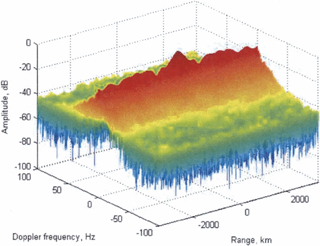
\includegraphics[width=0.6\textwidth]{AMspeechAmbSmall.png}
    \caption{Ambiguity Function of AM Signal \cite{AmbiguityCompare}}
    \label{fig:ambiguityAM}
\end{figure}

\begin{figure}[htbp]
    \centering
    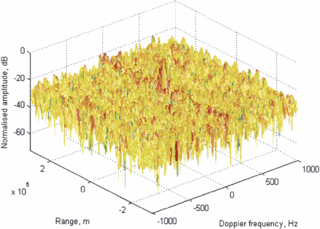
\includegraphics[width=0.6\textwidth]{drmPlotSmall.png}
    \caption{Ambiguity Function of DRM Signal \cite{AmbiguityCompare}}
    \label{fig:ambiguityDRM}
\end{figure}

Whilst the bandwidth of both the above channels is relatively small, the ambiguity functions from Thomas et al. \cite{AmbiguityCompare} show aforementioned parameters.
  
\par \vspace{0.5cm} 
Illuminator signals are not limited to terrestrial signals, they can also include signals from satellites, and can be tailored to the specific requirements of the passive radar system. Benefits of satellite based illuminators include increased coverage area, and a more evenly distributed power density \cite{satelliteIlluminator}. An imporant distinction for satellite illuminators is the condition of geostationary orbit, resulting in negligible relative motion between the satellite and receiver. Another condition for satellite based illuminators is the requirement for high directional gain antennas, as the illuminator signal is transmitted from a satellite in geostationary orbit, which is approximately 35,786 km above the equator \cite{satelliteIlluminator}. Specifically, the satellite illuminator of interest is DVB-S, digital sattelite TV broadcast in the ku-band, which is a COFDM signal, with a bandwidth of 27-36MHz, and a typical power of 50-150W \cite{DVB-S}. Notably, the large broadcast bandwidth results in significant signal processing requirements, as shown by Yin et. al \cite{DVBnoise}.


\par \vspace{0.5cm}
\begin{table}[!ht]
    \centering
    \caption{Properties of Potential IoO's}
    \label{tab:rf_spectrum_management}
    \begin{tabular}{|p{3cm}|p{3cm}|p{3cm}|p{4cm}|}
        \hline
        \textbf{Broadcast network} & \textbf{Frequency band (MHz)} & \textbf{Transmitter bandwidth} & \textbf{Typical transmitter power (EIRP)} \\ \hline
        FM radio & 88–108 & 0–100 kHz & 10–100 kW \\ \hline
        DAB radio & 195–209 & 1.536 MHz & 1–10 kW \\ \hline
        DVB-T (television) & 177-227 & 7 MHz & 1–100 kW \\ \hline
        DVB-S (satellite) & 10.7-12.75(GHz) & 27–36 MHz & 50–150 W (transponder power) \\ \hline
    \end{tabular}
\end{table}


The above table highlights some key differences in broadcast signals, potential draw backs of utilising terrestrial digital signals include geographical constraints and low signal power in rural areas, along with multipath effects in urban and high reflective areas \cite{DTSO2009}. 

% \noindent A potential problem associated with the use of DAB as an illuminator is direct signal interference (DSI), with the effects being amplified in urban environments. Coleman et. al \cite{DABfeatures} explain that the sheer signal size of direct illuminator size relative to surveillance signal size results in a high level of DSI. They outline that the cross polarisation of the transmitted DAB signal can be utilised along with illuminator cancellation filtering to attain higher level suppression. The leakage of the illuminator signal into the target signal can be due to a range of factors including buildings, trees and other reflective items as highlighted by Palmer et. al \cite{DTSO2009}.

\par \vspace{0.5cm} 
\noindent Typical characteristics of Australian DAB+ signals include frequency of just over 200MHz, bandwidth of approximately 1.5MHz, and a minimal output power of 10kW effective radiated power (ERP), consequently covering a large area \cite{DABfeatures}. These digital signals employ a modulation scheme called COFDM (coded orthogonal frequency division multiplexing), which is a form of multi-carrier modulation that is robust against multipath interference \cite{INTRO2017}. COFDM works by dividing the signal into multiple, simultaneous streams which are orthogonal to each other, modulated at a different frequency, maximising robust signal propogation. This is particularly useful in the context of passive radar, as it allows for the target and reference signal to be received by the passive radar system even if it has been reflected off multiple surfaces, such as buildings or trees. More specifically, the Australian implementation of DAB+ is dictated by the ETSI standard EN 300 401, which specifies the modulation, coding and multiplexing of the signal \cite{etsi_DAB_standard}. DAB+ is encoded via the AAC+, with proper licensing required, the most commonly utilised forward error correction(FEC) is 3A \cite{DABaustralia}. At a high level, these protocols of DAB+ reflect a channel model which has encoding, modulation and noise handling (FEC) built in, which can be advantageous for passive radar systems. In summary, DAB along with other digital signals are advantageous for passive radar due to their wide bandwidth, constant envelope, and relatively high transmit power\cite{DABambiguity}. 

% \par \vspace{0.5cm} 
% \noindent All of the above features result in DAB signals being condusive for ambiguity function performance (analyzed in further detail below). This can mainly be attributed to the relatively wide bandwidth of DAB enabling good resolution, constant DAB envelope stemming from COFDM protocol, and the multipath resistance \cite{DABambiguity}. The above being said, every reason that DAB is appropriate for passive radar also extends to other digital illuminators of opportunity, such as DVB-T, which is also a COFDM signal, and has a higher bandwidth and power than DAB.



\section{Range Doppler Mapping}
Range doppler mapping is a technique used to determine the distance and relative velocity of targets by analyzing the frequency shift (Doppler shift) and time delay of the received signals after they are reflected off the targets. The signal response of a target at a particular range and velocity can be predicted by the ambiguity function seen in equation \ref*{eq:ambiguity} \cite{INTRO2017}. 
\begin{equation}
    \chi(\tau, f) = \int s_{\text{reference}}(t) s_{\text{received}}^*(t - \tau) e^{j2\pi f t} \, dt \label{eq:ambiguity}
\end{equation}

Where:
\begin{multicols}{2}
\begin{itemize}
\item \( \chi(\tau, f) \) is the ambiguity function.
\item \( \tau \) is the time delay.
\item \( f \) is the Doppler frequency.
\item \( s_1(t) \) is the transmitted signal.
\item \( s_2(t) \) is the received signal.
\item \( s_2^*(t - \tau) \) is the complex conjugate of the received signal, time-shifted by \( \tau \).
\item \( e^{j2\pi f t} \) is the complex exponential representing the Doppler shift.
\item The integral is taken over all time \( t \).
\end{itemize}
\end{multicols}

\noindent The ambiguity function can be plotted, thereby visualising resolution, sidelobe patterns and any discrepancies in range and doppler. This is especially important for passive bistatic radar, whereby waveforms are not explicitly designed for radar and the geometry also has an impact \cite{FundamentalsPassiveRadar}. Hughes visualises the geometry considerations and potential flaws of generic passive bistatic configuration below in Figure \ref{fig:ambiguity}.

\begin{figure}[htbp]
    \centering
    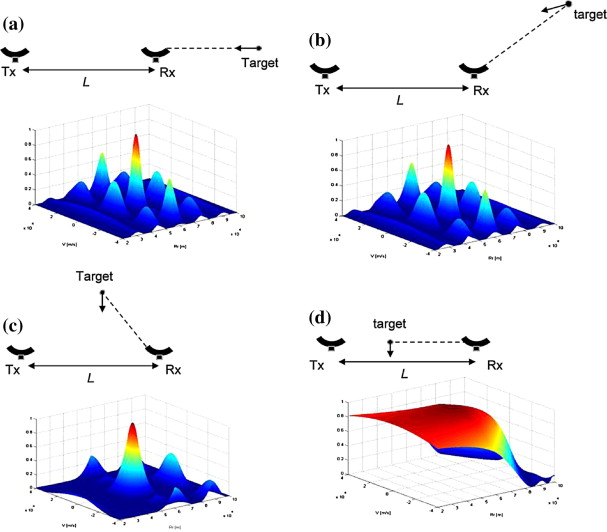
\includegraphics[width=0.7\textwidth]{ambiguity.jpg}
    \caption{Geometry and ambiguity function \cite{FundamentalsPassiveRadar}}
    \label{fig:ambiguity}
\end{figure}

\par \vspace{0.5cm} 
\noindent Understanding the link between geometric configuration and theoretical signal properties, the practical manifestation of the ambiguity function is range doppler mapping. As shown in Figure \ref{fig:rangeDoppler}, the map is a heat map and is derived with filters for noise minimsation, allowing for the visualisation of the target signal with minimal clutter. 

\begin{figure}[htbp]
    \centering
    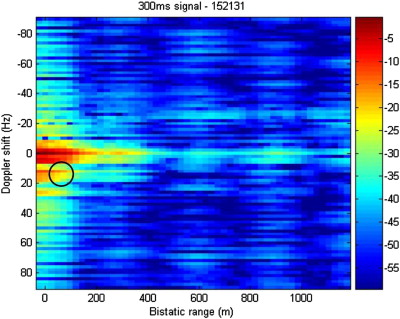
\includegraphics[width=0.6\textwidth]{rangeDoppler.jpg}
    \caption{Example of range doppler map for WiFi PBR \cite{FundamentalsPassiveRadar}}
    \label{fig:rangeDoppler}
\end{figure}


\par  
\noindent In the case of this project, the time delay will be utilised to calculate the bistatic range (x axis) and the Doppler shift will be used to calculate the relative velocity of the target (y axis). In summary, ambiguity function and subequent range doppler mapping will be vital for mapping the DAB+ signal characteristics for given geometry and motion of the surveilled target. \todo{MORE DETAIL}



\section{Radio Hardware}
Fundamentally, the relevant radio hardware for a passive radar project can be broken into the antenna and the SDR module. Given the low cost aims of this testbed, hardware cost and performance is a major consideration. 

\subsection{Software Defined Radio \label{sec: SDRdongle}}
Luckily, the proliferation of general purpose SDR hardware modules has enabled easy access to radio frequency (RF) signals \cite{SDRtheory}. In general, a SDR system can exist purely as a receiver (lower cost modules) or as a transceiver, whereby connected software (e.g. PC) are utilised for the modulation and demodulation of signals \cite{SDRgeneralInfo}. The SDR system can be used to sample the RF signal, and then process it digitally, enabling the use of a wide range of software tools for further signal processing. Typically, as seen in the block diagram below in figure \ref{fig:SDRblock}, SDR's comprise of an analogue front end, an analogue to digital converter (ADC) / digital to analagoue convertor (DAC), and some sort of band processing \cite{SDRgeneralInfo}.

\begin{figure}[htbp]
    \centering
    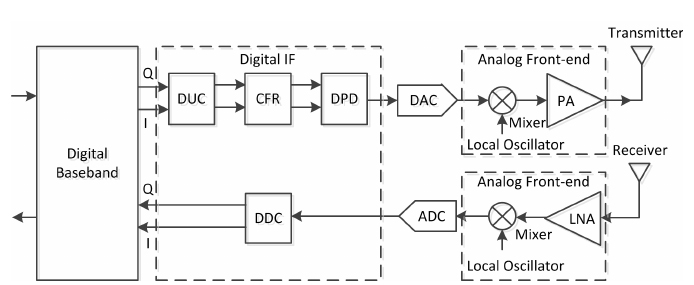
\includegraphics[width=0.8\textwidth]{sdrBlockDiagram.jpg}
    \caption{Block diagram of SDR transceiver \cite{SDRgeneralInfo}}
    \label{fig:SDRblock}
\end{figure}


\par \vspace{0.5cm}
The most popular and lowest cost SDR module is the RTL-SDR, which is a USB dongle that can be used to receive (note the RTL-SDR is RX only) and decode a wide range of RF signal bands. This includes FM radio, DAB, and DVB-T signals, which are all potential illuminators of opportunity for passive radar systems. Typical bandwidth of the RTL-SDR is 2.4MHz, and the frequency range is 24MHz to 1.7GHz \cite{SDRdongle}.

A plethora of other SDR modules exist, with varying costs and capabilities. A range of common SDR modules are listed in the table below \ref{tab:SDRcomparison}, along with their key specifications. 

\begin{table}[h!]
    \centering
    \caption{Comparison of SDR's \cite{SDRmoduleComparison} \label{tab:SDRcomparison}}
    \begin{tabular}{|l|l|l|l|l|}
    \hline
    \textbf{SDR} & \textbf{Frequency Range} & \textbf{Bandwidth} & \textbf{RX ADC} & \textbf{Sampling Rate} \\ \hline
    \textbf{USRP} & 0-6 GHz & Up to 160 MHz & 12-14 bits & Up to 200 MS/s \\ \hline
    \textbf{RTL-SDR} & 24 MHz - 1.75 GHz & Up to 2.4 MHz & 8 bits & Up to 3.2 MS/s \\ \hline
    \textbf{bladeRF} & 47 MHz - 6 GHz & Up to 56 MHz & 12 bits & Up to 61.44 MS/s \\ \hline
    \textbf{HackRF} & 1 MHz - 6 GHz & 20 MHz & 8 bits & Up to 20 MS/s \\ \hline
    \textbf{LimeSDR} & 0.1 MHz - 3.8 GHz & 61.44 MHz & 12 bits & Up to 61.44 MS/s \\ \hline
    \textbf{SDRplay} & 1 kHz - 2 GHz & Up to 10 MHz & 12 bits & Up to 10.66 MS/s \\ \hline
    \textbf{KrakenSDR} & 24 MHz - 1.76 GHz & Up to 2.5 MHz & 8 bits & Up to 2.56 MS/s \\ \hline
    \end{tabular}
\end{table}

As performance increases for the SDR's above so does the unit cost, which is an important consideration for the testbed design explored in scection \ref*{sec:hardware}. As seen in table \ref{tab:SDRcomparison}, other than the RTL-SDR all of the SDR's have a large bandwidth making them suitable for digital illuminators, furthemore, the ADC sampling bits are often larger, resulting in more more accurate signals. However, the increased resolution of an ADC also results in larger storage requirements and potentially bottlenecks in the processing chain \cite{SDRmoduleComparison}. Another interesting specification to note which is not seen on \ref*{tab:SDRcomparison} is the the number of RX channels. The RTL-SDR has one RX channel, whereas the USRP has two RX channels, which can be used to receive two signals simultaneously. This could be useful for the testbed, as it would allow for the simultaneous reception of the illuminator signal and the target signal, which could be used to improve the accuracy of the passive radar system. Specifically, the KrakenSDR features up to five channels, based on clustered RTL R820T2 tuners along with hardware to ensure the synchronisation of the channels \cite{KrakenSDR}. A key advantage of the KrakenSDR in passive radar receiver systems is their ability to achieve angle of direction measurements, which can be used to determine the location of the target as shown by Cass \cite{KrakenSDR}.

\subsection{Antenna \label{sec: antennaBackground}}
Quite simply defined by the IEEE as \textit{That part of a transmitting or receiving system that is designed to radiate or to receive electromagnetic waves} \cite{AntennaIEEE}, an antenna is crucial for any radio system, and in the case of passive bistatic radar, receiving all relevant signals. This section will provide a brief background of the key concepts and types of antennas relevant to passive bistatic radar. The ITEE standard definition of terms for antennas \cite{AntennaIEEE} also succinctly defines the following terms which are relevant;
\begin{enumerate}
    \item \textbf{Radiation Pattern}: This describes the angular variation in radiation at constant distances from the antenna. The radiation pattern depends on the signal strength and is categorized into three main types: Isotropic, Directional, and Omnidirectional.
    
    \item \textbf{Directivity}: Defined as the ratio of the power density in the direction of the pattern's maximum to the average power density at the same distance from the antenna. This can be measured through front to back ratio (dB), how well can antenna block signals from the rear.
    
    \item \textbf{Gain}: Closely related to directivity but includes losses. Gain is defined as the directivity minus any losses experienced by the antenna.
    
    \item \textbf{Polarisation}: This refers to the nature of the electric field radiated by the antenna. If the polarisation direction is not specified, it is assumed to be in the direction of maximum gain.
    
    \item \textbf{Bandwidth}: The range of frequencies over which the antenna operates effectively.
    
    \item \textbf{Beamwidth}: The angle between two points on the radiation pattern where the power is at its maximum. The two main types of beamwidth are Half Power Beamwidth (HPBW) and First Null Beamwidth (FNBW).
    
    \item \textbf{Impedance}: The ratio of voltage to current at the antenna terminals.
\end{enumerate}


As with considering the SDR module, the cost versus performance trade-off is also a key factor when selecting an antenna. The most common types of antennas used in passive radar systems are the dipole antenna and the Yagi-Uda antenna. The dipole antenna is a simple, low-cost antenna that is easy to construct and has a wide bandwidth. The Yagi-Uda antenna is a more complex, directional antenna that has a higher gain and a narrower bandwidth. Given the utilisation of digital broadcast signals with relatively high power, a simple dipole antenna may be sufficient for the testbed, however, the Yagi-Uda antenna may be required for more complex applications. High gain directional antennas can be chained together to receive signals from all directions, and in a passive radar context, determine the direction of the target \cite{KrakenSDR}.


\section{Digital Signal Processing}
Broadly, the goal of the signal processing for general passive bistatic radar is to extract a range doppler map from a received signal. Obtaining a range doppler map involves a few steps, with specifics depending on the IOO chosen along with number of sampling channels. Furthermore, there is the option of autocorrelating these signals via correlation integrals which is the most time and compute intense, or through Batches algorithm in the frequency domain \cite{IOTpassiveRadar}. Prior to the advent of of digital broadcasts, analague broadcast processing involved comprehensive filtering and synchronisation of at least two input channels\cite{DSPfm}. However, more recently, given the nature of DAB / DVB-T and its COFDM modulation, filtering and synchronisation can be replaced with reconstruction of the surveillance signal \cite{DSPdab}, replacing the need for dual channel configuration. Fundamentally, the single channel version of this correlation is the direct signal (given its strength) compared with a time lagged version of itself given the refelection from the target, as reflected in \ref{eq:ambiguity}. Mahfoudia, et al. demonstrate the methodology behind single channel correlation and reconstruction with a DVB-T illuminator, combined with clutter suppression techniques \cite{singleChannel}. For radar systems, as opposed to communication systems, the contents and packet structure of the signal is not necessarily relevant, rather the similarities of signals \ref{eq:ambiguity}.


The simplest, yet probably most computationally intense method of processing the doppler map is via traditional FFT-based correlation. It works by correlating large portions of the signal in time and frequency domains, with doppler shifts applied, creating frequency bins which are used to correlate with the received signal in the frequency domain, thereby obtaining any doppler shift experienced by the target. As for the time domain, the range estimates of a target can be obtained by taking the inverse fast fourier transform (IFFT) of the correlated signal in the frequency domain, providing the relevant time delay (and therefore range). The process can be repeated over multiple windows of a given signal and then combined to create a range doppler map \cite{FFTcorrelation}.

% ADD ANOTHER IMAGE??? --> Processing chain from Poster


\par \vspace{0.5cm} 
\noindent The computationally intense FFT correlation method can be refined and optimised by taking slow time 'batches', reducing the size of required FFT calculations. Once the signal has been received and windowed, according to Moser et. al, a FFT the size of 2048 for the range domain and 512 for the doppler domain can be computed \cite{IOTpassiveRadar}, see Figure \ref{fig:FFT}. 

\begin{figure}[htbp]
    \centering
    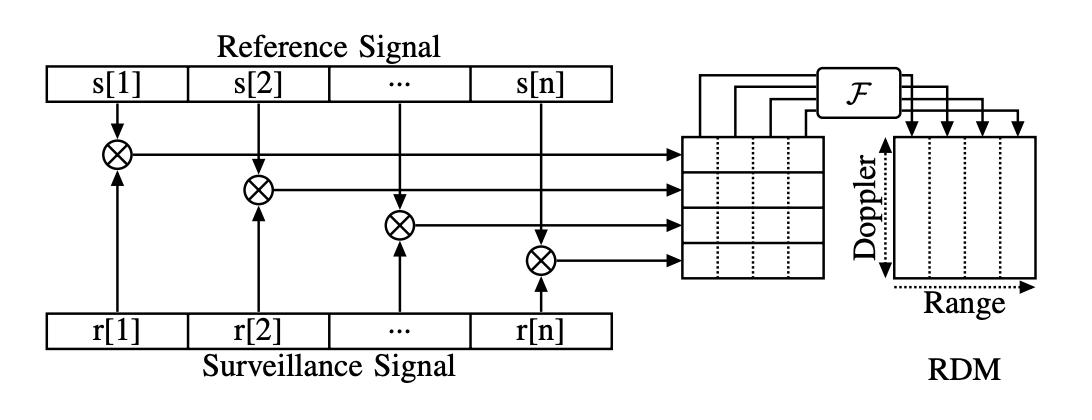
\includegraphics[width=0.8\textwidth]{FFT.png}
    \caption{Correlation and FFT for Range Doppler Mapping \cite{IOTpassiveRadar}}
    \label{fig:FFT}
\end{figure}

Given that single channel configurations are vulnerable to noise, interference and multipath, the outputs of pure correlation can result in clutter on the range doppler map. In the case of single channel configuration for PBR, the signl from the target (already quite weak) can be obstructed by unwanted reflections from buildings, trees, and other objects \cite{INTRO2017}. The above algorithms can be combined with a decluttering chain, which can implement something along the lines of a weiner filter, or a matched filter, to remove unwanted signals from the range doppler map \cite{FundamentalsPassiveRadar}. The implementation of clutter suppression algorithms, specifically background mean subtrafction (BMS) and guard mean substraction (GMS) has been shown by Zhang et al, working to clear up range doppler maps \cite{ZhangClutter}. This clutter suppression is especially neccessary around low doppler shift targets, as the clutter can be mistaken for the target signal. The presence of clutter given lack of suppression can be seen in Figure \ref{fig:clutter} below (yellow higher intensity pixels).

\begin{figure}[htbp]
    \centering
    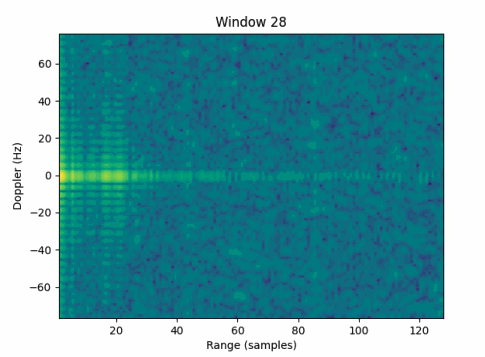
\includegraphics[width=0.6\textwidth]{clutterRDM.png}
    \caption{Clutter suppression (lack of) in range doppler map, taken from testing area with no target}
    \label{fig:clutter}
\end{figure}


\noindent Logically, the process above relfects the most computationally intensive step of the project ... hence, considerations with regard to signal processing algorithms will need to be taken in order to keep the overall detection system low cost, despite it not being a major factor of the testbed creation itself. 


\section{IoT Architecture}

The IoT architecture in the scope of this project refers to the computational platforms utilised to undertake the digital signal processing which then maps to tracking and detection of the target. At a high level, ITEE defines the Internet of Things (IoT) as \textit{"as a world of interconnected things that are capable of sensing, actuating, and communicating among themselves and with the environment ... provides the ability to share information and autonomously respond to real/physical world events by triggering processes and creating services with or without direct human intervention"} \cite{IoTdefinition}. In terms of PBR, existing studies have demonstrated the ability of off the shelf laptops \cite{FMlowCost}, and there is a few studies that use IoT platforms for FM signal processing \cite{IOTpassiveRadar}. The vital consideration when exploring hardware are the DSP and sampling requirements for a given illuminator signal and antenna configuration. More broadly, IoT hardware has been used in a range of general tracking and detection applications. A prime example of this is the Flightradar24 service which utilises a network of ADS-B receivers to track aircraft in real time, where they provide a hardware kit of a Raspberry Pi and a DVB-T dongle (RTL-SDR) \cite{flightradar24}, channelling the data to a central server for processing and mapping. 

\par \vspace{0.5cm} 
\noindent According to Schupbach et. al \cite{DABprocessingChain}, the broad scope capability requirements of the computational platform and associated processing can be grouped into signal acquisition, signal reconstruction and then the correlation function calculation. With a single board computer, this can be largely achieved through a combination of software libraries along with python script, however the hardware facilitating this processing is a key consideration. Largely, the IoT hardware is limited to single board computers, as microcontroller units (MCU) are not capable of the sampling and detection processing requirements, along with the fact that the project requires a full operating system for relevant SDR libraries. Exploring other potential architecture such as FPGA's, again are not as well suited, given their high cost and complexity, although their is precedent for the signal processing and recording \cite{FPGAhardware}. A range of single board computers are available, and can be compared primarily based on their processing power, memory / memory access, and cost \cite{sbc_hardware}, as viewed in the table below.

\begin{table}[h!]
    \centering
    \begin{tabularx}{\textwidth}{|p{3cm}|X|X|X|X|X|p{2cm}|}
    \hline
    \textbf{SBC} & \textbf{CPU} & \textbf{RAM} & \textbf{Storage Access} & \textbf{OS Support} & \textbf{Size (mm)} & \textbf{Price (USD)} \\
    \hline
    \textbf{Raspberry Pi Zero 2 W} & Quad-core Cortex-A53, 1 GHz & 1GB & microSD & Raspberry Pi OS, Linux & 65 x 30 & 15 \\
    \hline
    \textbf{Raspberry Pi 4} & Quad-core Cortex-A72, 1.5 GHz & 2/4/8GB & microSD, USB & Raspberry Pi OS, Linux & 85.6 x 56.5 & 35-75 \\
    \hline
    \textbf{Raspberry Pi 5} & Quad-core Cortex-A76, 2.4 GHz & 8GB & microSD, PCIe (through HAT), USB & Raspberry Pi OS, Linux & 85.6 x 56.5 & from 60 \\
    \hline
    \textbf{Nvidia Jetson Nano} & Quad-core Cortex-A57, 1.43 GHz & 4GB & microSD, PCIe (through adapter) & Ubuntu, JetPack & 100 x 80 & 100 \\
    \hline
    \textbf{Orange Pi 5} & Octa-core Cortex-A76/A55, 2.0 GHz & 8GB & eMMC, microSD, PCIe & Android, Linux & 90 x 60 & 80 \\
    \hline
    \end{tabularx}
    \caption{Comparison of Single Board Computers \cite{sbc_hardware}}
    \label{tab:sbc_comparison}
    
\end{table}


\par \vspace{0.5cm} 
\noindent There is precedent of previous use for the Raspberry Pi platform as demonstrated by Moser et. al \cite{IOTpassiveRadar} An alternate, higher powered choice in which Sednall demonstrated is the higher powered Nvidia Jetson, which includes faster processing times due to its quad core architecture \cite{FMlowCost}. The price for these options is \$60 compared to \$250 respectively. Ultimately, the choice of embedded IoT hardware for the project can be reduced to the trade off between low cost and processing power, and will be a key consideration in the project plan. Furthermore, there is possibility to design custom hardware or utilise the GPIO functionality of the single board computer, as reflected by the high level definition of IoT architecture by ITEE \cite{IoTdefinition}.

\section{Networking with Embedded Hardware}

Given that the overall goal of this thesis project is to create a low cost, embedded passive radar detection system, valuable to consider how this would be visualised, be it via wired or wireless protocol. Essentially, depending on whether the RDM is computed on the 'edge' (ie embedded device) or on a PC, the networking requirements will differ. For example, if it is only IQ sampling completed on the embedded testbed platform, only the IQ data in the form of a .bin file needs to be transferred, however, if the RDM is computed on the embedded device, the entire RDM image / gif will need to be transferred. The following options vary in complexity and context, but all facilitate the relavant transfer of data from the embedded device to a PC for further processing or visualisation.

\subsection{USB Drive Transfer}
The most basic method of transferring data from an embedded device to a PC is via a USB drive. This method is simple and reliable, and is ideal for applications where the data transfer rate is not critical. The data is saved to a USB drive on the embedded device, and then transferred to a PC for further processing. However, it is not ideal for real-time applications, as the data transfer is limited by proximity and a manual process is required (despite large data storage capabilities).

\subsection{SSH}
Secure Shell (SSH) is a widely-used method for remotely interfacing with embedded devices and SBC's. It allows users to securely log in to a remote device over a network and issue commands as though they were operating directly on the device. This is particularly useful for headless systems, where the embedded device does not have a monitor or keyboard connected. SSH encrypts all communication, ensuring data security. Once an SSH connection is established between the Raspberry Pi and a PC, tasks such as starting data capture, configuring parameters, or transferring files can be done directly from the PC terminal \cite{SSHOverview}. Many applications use SSH for remote monitoring and control of embedded systems, as well as for viewing the UI of SBC's, for example VNC viewer.


\subsection{Ethernet}
Ethernet is one of the most common and reliable methods for data transfer between embedded systems and PCs, offering high data transfer speeds and low latency. Ethernet is a wired networking technology that forms the backbone of local area networks (LANs). It supports high-speed data transmission, typically at 100 Mbps (Fast Ethernet) or 1 Gbps (Gigabit Ethernet) \cite{rpi5_wifi}, making it a suitable for applications that require real-time data transfer or when working with large datasets, such as IQ samples or RDM files. Ethernet uses a network cable (e.g., CAT5, CAT6) to connect devices in a LAN. It transmits data packets using the Internet Protocol (IP), allowing connected devices to communicate with one another. The data packets are routed through switches and routers, which direct the flow of traffic within the network. Ethernet is widely used in industrial automation, IoT, and other applications that require reliable and high-speed data transfer.

\subsection{TCP Socket}
A TCP (Transmission Control Protocol) socket is a software-based method for creating a reliable connection between two devices over a network. TCP ensures that all data packets are transmitted in the correct order and without loss, making it ideal for real-time data streaming applications such as radar data. In the case of this project the testbed would act as the client, initiating data transfer to the server (PC). This can be implemented over a wireless network \cite{TCPoverview}.

\subsection{Cloud Service}
Another modern solution for data transfer between embedded devices and PCs is the use of cloud services. The embedded testbed can upload data to cloud storage, which can then be accessed from the MacBook Air, or vice versa. An obvious downside of this method is the reliance on an internet connection, and the potential for data security issues. 





% \begin{figure}[h]
%     \centering
%     
\includegraphics[width=0.25\textwidth]{UQLogo.png}
%     \caption{An Example Image}
%     \label{fig:uq}
% \end{figure}